
\subsection{Estimación del nivel y potencia por Monte Carlo}

Para estimar el nivel y la potencia de cada test se repite $R$ veces el siguiente experimento: (i)~generar $X_1,\dots,X_n$ i.i.d.\ de la distribución de interés; (ii)~calcular el p-valor $p_r$ del test mediante $B=199$ remuestras bootstrap de $sF_n(\hat\theta)$; (iii)~registrar $I_r=\mathbf{1}\{p_r\le\alpha\}$. La tasa de rechazo empírica
\[
\hat\pi_n \;=\; \frac{1}{R}\sum_{r=1}^{R} I_r
\]
estima el error Tipo I bajo $H_0$ o la potencia bajo $H_a$, con error estándar $\sqrt{\hat\pi_n(1-\hat\pi_n)/R}$. Se fijó $\alpha=0.05$, y se usaron $R=300$ réplicas para $T_n$ y $R=200$ para $S_n$.

\begin{observacion}
El p-valor $\hat p=\bigl(1+\#\{b:T_n^{*(b)}\ge T_n\}\bigr)/(B+1)$. Para rechazar a nivel $\alpha$, se requiere que $\p( p\leq \alpha) = \alpha$, bajo la validez del bootstrap, $p(B+1)$ es aproximadamente uniforme en $\{1,...,B+1\}$. Es decir, $\p( p \leq \alpha) = \p(p(B+1) \leq \alpha(B+1)) = \sum_{i=1}^{\lfloor \alpha(B+1) \rfloor} \frac{1}{B+1} = \frac{\lfloor \alpha(B+1) \rfloor}{B+1}.$ Para poder rechazar a nivel $\alpha$ exacto basta pedir $\alpha\cdot(B+1) \in \N$.

Por otro lado,  como $\hat{p}\in \{\frac{1}{B+1},...,1\}$ esto introduce un sesgo de discretización pues obliga a nuestra estimación a saltar en escalones de $\frac{1}{B+1}$. Para que este riesgo sea despreciable en comparación al la desviación estándar del Montecarlo ($SE_R= \sqrt{\frac{0.05\cdot0.95}{R}} \approx 0.0125 \approx 1.3 \%$. Pedimos que $\frac{1}{B+1}< 0.0125/2.$ Así, con $B= 199$ basta.
\end{observacion}


\subsection{Distribuciones}

Bajo $H_0$ se consideran dos distribuciones simétricas en $\theta=2$:
\[
X \sim \mathrm{Unif}(1,3), \qquad X \sim \mathrm{Cauchy}(2,1).
\]
Para medir potencia se consideran tres distribuciones asimétricas de cola derecha:
\[
X \sim \Gamma(k{=}2,\,s{=}1), \qquad X \sim \mathrm{Weibull}(k{=}1.5,\,s{=}1), \qquad X \sim \mathrm{Pareto}(a{=}3,\,s{=}1).
\]
Los tamaños de muestra son $n\in\{20,40,80,160\}$, elegidos para que la potencia muestre una transición clara de baja a alta conforme crece $n$.

\begin{figure}[H]
  \centering
  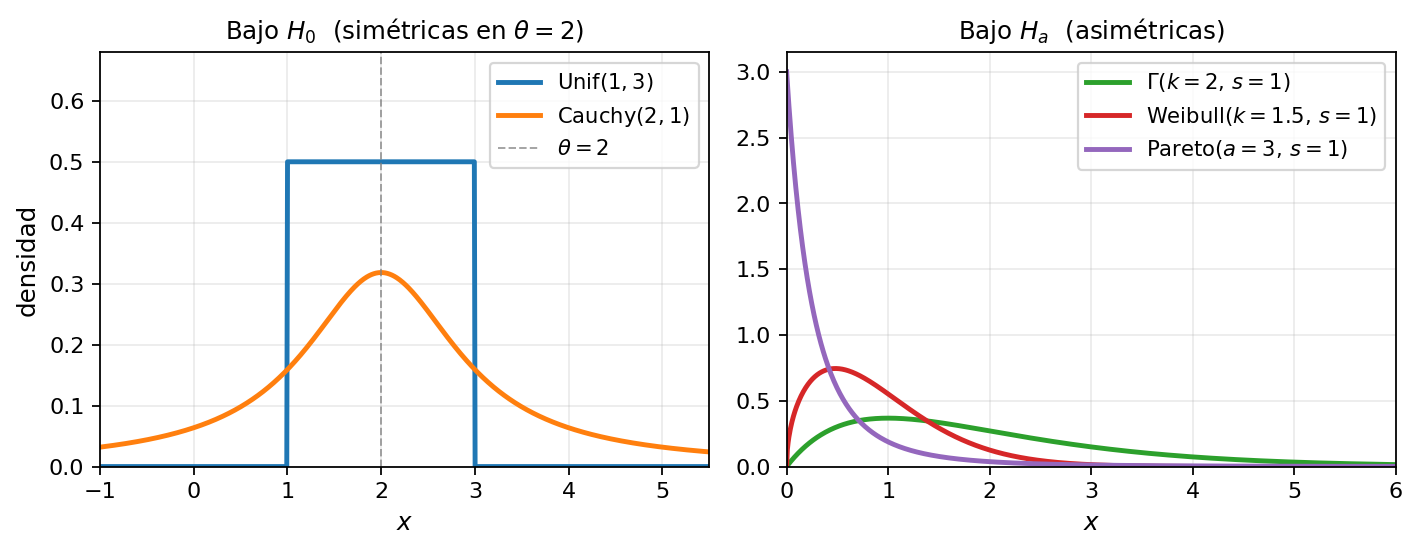
\includegraphics[width=0.92\textwidth]{../results/figures/densidades_distribuciones.png}
  \caption{Densidades de las distribuciones empleadas. Izquierda: $H_0$, ambas simétricas en $\theta=2$ (línea gris). Derecha: $H_a$, las tres con soporte $[0,\infty)$ y asimetría positiva, pero con distinto grado de curtosis y peso en la cola derecha.}
  \label{fig:densidades}
\end{figure}

\subsection{Estimadores del centro de simetría}

Se evalúan los tres estimadores de $\theta$ propuestos por Schuster y Barker~\cite{schuster1987bootstrap}:
\begin{itemize}

      \item $\hat\theta_{\mathrm{med}} = \mathrm{mediana}(X_1,\dots,X_n)$.
  
    \item $\hat\theta_\alpha = \bar{X}_{0.1}$: media afeitada con fracción $0.1$ en cada cola.
    
    \item $\hat\theta_{\min}$: minimizador de $T_n$ (resp.\ $S_n$). La Sección~\ref{sec:estim-theta} detalla los esquemas numéricos utilizados. Para $T_n$, se usa el algoritmo combinatorio exacto de Schuster-Narvarte (Sección~\ref{impl:argmin-Tn}) tanto sobre la muestra original como en cada remuestra bootstrap: las remuestras provienen de $sF_n(\hat\theta)$, que es exactamente simétrica, por lo que el algoritmo converge en pocas iteraciones y la búsqueda es exacta y eficiente.

    Para $S_n$, la Sección~\ref{sssec:grad-q1} demuestra que el estadístico es diferenciable en casi todo $\theta$ para $q=1$ y $q=2$, con gradientes analíticos cerrados (\eqref{eq:grad-Sn-q1} para $q=1$, \eqref{eq:grad-Sn} para $q=2$). En ambos casos se usa \texttt{L-BFGS-B} con gradiente analítico, lo que incluye la combinación $(q=1,\hat\theta_{\min})$ con el mismo esquema numérico que $q=2$. La Sección~\ref{impl:argmin-Sn} detalla la implementación.
\end{itemize}

\subsection{Funciones de peso para $S_n$}

La integral \eqref{eq:Sn} depende de $q$ y de $w$. Se consideran los dos exponentes $q\in\{1,2\}$ y tres densidades simétricas. Para $q=2$, el criterio es diferenciable respecto a $\theta$ y se usa el gradiente analítico de \eqref{eq:grad-Sn}. Para $q=1$, el integrando contiene una norma absoluta y a primera vista puede no ser diferenciable en los puntos donde \(c_n(t)e^{-it\theta}-|c_n(t)|=0\).
Sin embargo, la Sección~\ref{sssec:grad-q1} demuestra que $S_n$ es diferenciable en casi todo $\theta$ para $q=1$ —los ceros del seno forman un conjunto de medida cero en $t$ para cada $\theta$ fijo— y proporciona la fórmula cerrada~\eqref{eq:grad-Sn-q1}. Esto permite aplicar \texttt{L-BFGS-B} con gradiente analítico también para $q=1$, evaluando los tres estimadores del centro (mediana, media afeitada y argmin) en este caso.
\begin{align*}
  w_1(t) &= \frac{1}{\sqrt{2\pi}}\,e^{-t^2/2} & &(\mathcal{N}(0,1)),\\
  w_2(t) &= \frac{1}{0.5\sqrt{2\pi}}\,e^{-t^2/(2\cdot 0.5^2)} & &(\mathcal{N}(0,\,0.5^2)),\\
  w_3(t) &= \tfrac{1}{2}\,e^{-|t|} & &(\mathrm{Laplace}(0,1)).
\end{align*}
$w_1$ y $w_2$ difieren en el ancho de banda: $w_2$ concentra más masa en frecuencias bajas. $w_3$ tiene colas más pesadas que $w_1$ y pondera con mayor intensidad las frecuencias altas. La integral se aproxima por cuadratura trapezoidal en un grid de $K=301$ puntos adaptado al soporte efectivo de cada $w$.
